\documentclass[11pt]{article}

\usepackage[style=prsb,natbib=true,uniquename=false,uniquelist=false,sortcites=false]{biblatex}
\addbibresource{refs.bib}

\usepackage{graphicx}
\usepackage{xcolor}
\usepackage{booktabs}
\usepackage{array}
\usepackage[letterpaper]{geometry}
\geometry{hmargin={1in,1in},vmargin={0.7in,0.7in}}

\usepackage[hidelinks]{hyperref}
\usepackage[inline]{enumitem}
\newlist{ilnum}{enumerate*}{1}
\setlist[ilnum]{ label=(\Roman*) }

\usepackage{amsmath}
\usepackage{amsthm,amssymb}
\usepackage{mleftright}
\mleftright


%%%%%%%%%%%%%%%%%%%%%%%%%%%%%%%%%%%%%%%%%%%%%%%%%%%%%%%%%%%%%%%%%
% XeLaTeX font settings
\usepackage{fontspec}
\defaultfontfeatures{Ligatures=TeX}
\usepackage{unicode-math}

\setmainfont{Minion Pro}
\setsansfont[Scale=MatchLowercase]{Myriad Pro}
\setmonofont[Scale=MatchLowercase]{Fira Code}
\setmathfont[Scale=MatchLowercase]{TeX Gyre Pagella Math}
\setmathfont[range=up/{num,latin,Latin,greek,Greek}]{Minion Pro}
\setmathfont[range=it/{latin,Latin,greek,Greek}]{Minion Pro It}
\setmathfont[range=bfup/{latin,Latin,greek,Greek}]{Minion Pro Bold}
\setmathfont[range=bfit/{latin,Latin,greek,Greek}]{Minion Pro Bold It}
%%%%%%%%%%%%%%%%%%%%%%%%%%%%%%%%%%%%%%%%%%%%%%%%%%%%%%%%%%%%%%%%%

\usepackage[explicit]{titlesec}
\titleformat{\section}        {\large \bfseries \scshape}{\thesection.}{1ex}{#1}
\titleformat{\subsection}     {\bfseries \itshape}{\thesubsection.}{1ex}{#1}
\titleformat{\subsubsection}  [runin]{\bfseries}{\thesubsubsection.}{1ex}{#1}

\titlespacing{\section}       {0pt}{1.5ex plus 0.5ex minus 0.5ex}{0.5ex plus 0.5ex minus 0.5ex}
\titlespacing{\subsection}    {0pt}{1.5ex plus 0.5ex minus 0.5ex}{0.0ex plus 0.25ex minus 0.25ex}
\titlespacing{\subsubsection} {0pt}{1.5ex plus 0.5ex minus 0.5ex}{1em}

\usepackage{setspace}
\usepackage{titling}
\usepackage{xparse}
\usepackage{lineno}

\usepackage{tikz}
\usetikzlibrary{arrows}

%%% new commands and macros

\newcommand{\der}{\mathop{}\!\mathrm{d}}
\newcommand{\Oh}[1]{O\left(#1\right)}
\newcommand{\ExpectationOperator}{\mathrm{E}}
\NewDocumentCommand \E {d[] d()} {%
  \IfNoValueTF {#1} {%
    \IfNoValueTF {#2} {%
      \mathop{\kern0pt\ExpectationOperator}\nolimits%
    }{%
      \mathop{\kern0pt\ExpectationOperator}\nolimits\left(#2\right)%
    }}{%
    \IfNoValueTF {#2} {%
      \mathop{\kern0pt\ExpectationOperator#1}\nolimits%
    }{%
      \mathop{\kern0pt\ExpectationOperator#1}\nolimits\left(#2\right)%
    }%
  }
}
\DeclareMathOperator{\Var}{Var}
\DeclareMathOperator{\Cov}{Cov}
\newcommand{\Fst}{F_{\mathrm{ST}}}
\newcommand{\mean}[1]{\overline{#1}}
\newcommand{\w}{w}
\newcommand{\ess}[1]{#1^*}
\newcommand{\fixp}[1]{\hat{#1}}
\renewcommand{\vec}[1]{\symbf{#1}}
\newcommand{\rec}{\rho}
\newcommand{\mut}{\mu}

\newtheorem{result}{Result}

\newcommand{\xaxisandtickspip}{
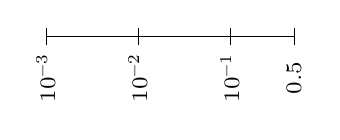
\begin{tikzpicture}[>=angle 90,scale=1.05]
  % x-axis
  \draw[] (0,0)--(3,0);
  % Tick marks and annotations
  %\path (1.5,-0.8) node [below]{$\mu_M$};

  \foreach \x/\nodeLabel in {0/$10^{-3}$,
    1.1115/$10^{-2}$,
    2.2231/$10^{-1}$,
    3/$0.5$}
  {
    \draw (\x,-0.1) -- (\x,0.1);
    \path[anchor=center] (\x,-0.5) node[rotate=90] {\footnotesize\nodeLabel};
  }
\end{tikzpicture}
}

\newcommand{\yaxisandtickspip}{
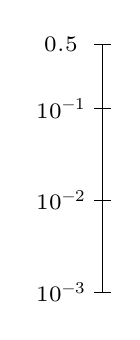
\begin{tikzpicture}[>=angle 90,scale=1.05]
  % y-axis
  \draw[] (0,0)--(0,3);
  % Tick marks and annotations
  %\path (-0.8,1.5) node [left]{$\mu_m$};

  \foreach \y/\nodeLabel in {0/$10^{-3}$,
    1.1115/$10^{-2}$,
    2.2231/$10^{-1}$,
    3/$0.5$}
  {
    \draw (-0.1,\y) -- (0.1,\y);
    \path[anchor=center] (-0.5,\y) node {\footnotesize\nodeLabel};
  }
\end{tikzpicture}
}

%%%

\begin{document}

\begin{titlingpage}
\setlength{\droptitle}{2em}
\pretitle{\begin{center}\LARGE}
\posttitle{\par\end{center}\vskip 2.5em}

\title{\scshape Evolutionary dynamics, equilibrium selection, and what population and quantitative genetics have taught evolutionary game theory}
\author{Jeremy Van Cleve}
\date{}
\maketitle

\vfill

\noindent
Department of Biology\\
University of Kentucky\\
Lexington, KY 40506 USA\\[1em]
phone: 859-218-3020\\
fax: 859-257-1717\\[1em]
e-mail: \href{mailto:jvancleve@uky.edu}{jvancleve@uky.edu}

\vspace{2em}

\begin{flushright} \textit{Date modified: \today} \end{flushright}
\end{titlingpage}

\linenumbers
\onehalfspacing
\begin{abstract}

The application of game theory to animal behavior by Maynard Smith and Price invigorated evolutionary biology by suggesting that the complex dynamics among natural selection, genes, and behavior could be analyzed using an evolutionary refinement of the Nash equilibrium, namely the evolutionarily stable strategy (ESS)\@. As implied by ``equilibrium'' and ``stable'', an ESS is a predicted long-term outcome that an evolutionary process may reach via natural selection and mutation. ESS analysis has been particularly important in highlighting the importance of social dilemmas in biology where the evolution of cooperative behavior can be undermined by the individual fitness costs of that behavior. However, even simple games like the stag-hunt or coordination game can have multiple ESSs, which begs the question, which ESS is more likely to evolve? Unfortunately, ESS analysis does not reveal which ESS is more likely to evolve nor does it even show how genetic or demographic factors affect the speed of approach to an ESS. Progress on determining which ESSs are more ``realistic'' has been made using tools from stochastic processes and population and quantitative genetics including stochastic stability, absorption times, and G-matrix theory. In this paper, we will review the use of these tools and provide novel insight into how they can predict social evolution as a function of genetic and demographic processes.

\end{abstract}

\vspace{3em}
\noindent {\bfseries Key words}\\

\newpage

\section{Outline/Brainstorm}

\begin{enumerate}
  \item Intro
        \begin{enumerate}
          \item Little intro about Maynard Smith and Price
          \item Game theory as general optimization and search for fixed points
          \item Connect back to Hamilton 1964 and goal of optimization with relatedness
          \item Evolutionary process is dynamic but still has ``fixed points''
          \item Evolutionary change can be decomposed and each piece affects location and stability of fixed points
          \item Evol Game theory captures selection but not demography and genetic forces, which can have strong effects.
        \end{enumerate}
  \item Ok, so thinking more about this, the two main pieces in certain ways are the fitness or success measure and whether maximizing it leads a correct predictions. pop mean fitness as measure fails due to genetics and due to frequency dependence. hamilton suggested inclusive fitness. later authors showed that this is equivalent to an invasion fitness perspective. maximization of this leads to ESS. Stochasticity though due to mutation/drift/etc leads to stationary distribution...
  \item Extra things
        \begin{enumerate}
          \item emphasize the incompleteness of the review. Maybe cite a few ``relevant'' Perc papers?
        \end{enumerate}
\end{enumerate}

%%
the flow for the intro should be something like: maynard smith setup this false dichotomy: ESS is about ``individual'' level selection when really there are two issues, ESS as tool of optimality and then the application of that tool to kin/group models. this requires explaining how ESS is a tool of optimality and how a particular optimality measure, namely lineage growth rate, accounts for kin and group selection since it can captures selection at all levels from the gene on up. accounting for other evolutionary forces is more difficult but one way forward uses the fixation probability and allows mutation/demography etc to affect fixation probabilities and hence transition rates.


\clearpage
\section{Introduction}

Although Richard Lewontin was the first to introduce game theory into biology in 1961 \cite{Lewontin:1961}, very few papers on the topic of game theory and biology were published in the following decade. It wasn't until 1973 when John Maynard Smith and George Price introduced the evolutionarily stable strategy (ESS) and applied it to the study of animal behavior \cite{Maynard-Smith:Price:1973} that biologists more widely came to appreciate the relevance and utility of game theoretic concepts and tools for questions in evolution biology and ecology. Specifically, Maynard Smith and Price posited that individual fitness could be viewed as an analog of the game-theoretic notion of ``utility'', which is the quantity that measures what agents optimize in pursuit of their objectives \cite{Myerson:1991}. Viewed this way, the ESS is a refinement of the famous Nash equilibrium \cite{Nash:1950}. Maynard Smith explained the ESS concept in more detail in an important paper in 1974 \cite{Maynard-Smith:1974}, introduced the famous ``Hawk-Dove'' game in his study of asymmetric games in 1976 \cite{Maynard-Smith:Parker:1976}, and summarized the nascent field of evolutionary game theory in his now classic 1982 book \cite{MaynardSmith:1982}. In the 50 years since the 1973 paper, evolutionary game theory has become an essential tool in evolutionary and behavioral ecology with rich theoretical work that delves into foundational evolutionary and game-theoretic concepts and mathematical and simulation models that predict ESSs for almost innumerable biological systems. Evolutionary game theory has also strongly influenced the social sciences including, naturally, economics, political science, psychology, and anthropology and has drawn applied mathematicians, computer scientists and physicists into mathematical biology.

The role of evolutionary game theory and the ESS method specifically in evolutionary biology has been at the crux of some of the most important conceptual debates in the field including the role of natural selection and adaptation vis-a-vis other forces \cite[e.g.,][]{MaynardSmith:1978,Gould:Lewontin:1979,Lewontin:1979,Orzack:Sober:1994,Gardner:2017,Kern:Hahn:2018,Jensen:Payseur:2019} and the importance of kin and group selection relative to individual selection
\cite[e.g.,][]{Maynard-Smith:1964,Hamilton:1963,Price:1972:cov,Wilson:Wilson:2007,Leigh:2010,Akcay:VanCleve:2012,West:Griffin:2007,Gardner:Grafen:2009,Nowak:Tarnita:2010,Abbot:Abe:2011,Allen:Nowak:2013,Birch:2014,Birch:2017,Nowak:McAvoy:2017}. These debates might be captured in part by the following two questions: \begin{ilnum} \item \label{q:I} How do ESS models that focus on individual fitness capture the effects of kin selection or group selection? \item \label{q:II} How does an ESS account for mutation, genetic drift, and other evolutionary forces? \end{ilnum} In this work, I will describe how conceptual advances in evolutionary theory since Maynard Smith and Price \cite{Maynard-Smith:Price:1973} have shed light on both of these questions and have led to a broader understanding of the ESS method and a more integrative framework for understanding how multiple evolutionary forces in complex populations can lead to diverse phenotypes.

Question \ref{q:I} derives in part from how Maynard Smith introduced his work on ESSs; he argued that an ESS could provide an explanation for the evolution of behaviors where ``selection acts entirely at the individual level, but in which the success of any particular strategy depends on what strategies are adopted by other members of the population'' \cite[][p. 210]{Maynard-Smith:1974} and is not ``due to group or species selection'' \cite[p. 15]{Maynard-Smith:Price:1973} or selection on ``close relatives'' \cite[p. 210]{Maynard-Smith:1974} as might be the case for kin selection \cite{Hamilton:1964}. In setting up this dichotomy, Maynard Smith implies that the ESS method may not apply when kin or group selection are involved and that kin or group selection models might lead to different results when applied to the same biological scenario. As I will describe below, evolutionary theorists have since realized (including Maynard Smith himself \cite[p. 33]{MaynardSmith:1978}) that the ESS method is really orthogonal to issues of individual vs. group vs. kin selection and instead captures in what sense evolution via natural selection optimizes fitness given a specific measure of fitness. Issues of individual vs. group vs. kin selection are about the ``units'' or ``levels'' at which selection acts and how fitness should be measured to account for selection at those levels. Lewontin also hints at the levels of selection question in his 1961 game theory paper when he discusses the relative merits of individual-level measures of fitness like intrinsic or Malthusian growth rate $r$ versus population-level measures like mean fitness $\mean{w}$ \cite[p. 400-401]{Lewontin:1961} as analogs of utility. The levels of selection question became a major topic of study in evolutionary theory \cite[e.g.,][]{Lewontin:1970,Dawkins:1982,Wilson:Sober:1989,Maynard-Smith:Szathmary:1995,Wilson:1997,Michod:1999,Michod:2006,Szathmary:2015} and philosophy of biology \cite{Hull:1980,Brandon:1982,Damuth:Heisler:1988,Lloyd:1992,Lloyd:1994,Sober:Wilson:1994,Okasha:2006,Okasha:2016} and continues to generate substantial research \cite[e.g.,][]{Black:Bourrat:2020,Cooney:Mori:2022,Veit:2022}. For the purpose of explaining how an ESS can capture selection at multiple levels and among relatives or kin, I will argue below that the right measure of utility is the ``lineage fitness'' \cite{Lehmann:Alger:2015,Akcay:VanCleve:2016,Lehmann:Mullon:2016} of a mutant allele at a single genetic locus, which can be shown to be functionally equivalent to a measure of inclusive fitness \cite{Lehmann:Mullon:2016,Lehmann:Rousset:2020}.

The origin of question \ref{q:II} rests in a different set of debates in evolutionary biology regarding the relative role of natural selection vis-a-vis other evolutionary forces, such as mutation, recombination, and gene flow, in explaining organismal phenotypes. Early in the 20th century, R. A. Fisher's ``fundamental theorem of natural selection'' (FTNS) \cite{Fisher:1930} established a mathematical expression of the importance of natural selection. The FTNS states that the increase in the mean fitness of a population is equal to the genetic variance in fitness and thus seems to imply that populations always become better adapted to their environments and even that fitness is maximized over the long term. It's hard to overstate the importance of the FTNS in shaping the direction of evolutionary theory. The FTNS came to typify the idea that evolutionary change is dominated by natural selection as a fitness optimizing force. Bill Hamilton appealed to this idea in his original paper on kin selection \cite{Hamilton:1964} and theorized that ``inclusive fitness'' is the fitness quantity that is maximized.

Subsequent work by population geneticists revealed however that mean fitness can decrease due to frequency-dependent selection \cite{Wright:1955,Lewontin:1970} or recombination among multiple genetic loci \cite{Kojima:Kelleher:1961,Moran:1964,Karlin:1975,Akin:1979}. Further, studies in the 1960s of the rates of molecular evolution \cite{Zuckerkandl:Pauling:1965,King:Jukes:1969} and levels of polymorphism \cite{Harris:1966,Lewontin:Hubby:1966} in a number of species spurred the development of the neutral \cite{Kimura:1968,Kimura:1983:book} and nearly neutral \cite{Ohta:1974,Ohta:1992} theories \cite{Ohta:Gillespie:1996} of molecular evolution. These theories posited that many mutations are weakly affected by natural selection, and thus their fate is governed mostly by genetic drift \cite{Kimura:1983:book}. Consequently, by the 1970s, evolutionary biologists were heavily debating both the relative role of natural selection versus other forces in shaping evolutionary patterns \cite{Gillespie:Langley:1974,Gillespie:1978}, and some biologists including Lewontin specifically questioned the importance of fitness maximization \cite{Karlin:1975,Gould:Lewontin:1979}. Maynard Smith was a clear proponent of fitness maximization and viewed it natural to ``[assume] that evolution has occurred by natural selection'' \cite[p. 31]{MaynardSmith:1978}. Thus, he proposed the ESS method developed by Price and himself as the appropriate tool for predicting phenotypic evolution and particularly for social traits. While Maynard Smith acknowledged that ESS models make a number of biological assumptions including that traits have a simple genetic basis (i.e., no dominance, epistasis, etc) and that appropriate genetic variation exits \cite{MaynardSmith:1978}, he believed that the limitations imposed by these assumptions are reasonable. This view that simplifying away genetic complexities or constraints is generally reasonable was termed the ``phenotypic gambit'' by Alan Grafen \cite{Grafen:1984} and came to dominate evolutionary theory in behavioral and evolutionary ecology \cite{Houston:McNamara:1999}. The near-singular focus of evolutionary game theory and the ESS method on natural selection has become less defensible given the recent and increasing abundance of genomic and transcriptomic data for a diverse set of species \cite[e.g.,][]{Kapheim:Pan:2015,Mikheyev:Linksvayer:2015,Warner:Mikheyev:2017,Kocher:Mallarino:2018,Warner:Mikheyev:2019}; specifically, some have argued that understanding these data requires moving beyond the gambit with more explicit consideration of complex genetic and demographic mechanisms \cite[e.g.,][]{Springer:Crespi:2011,Rittschof:Robinson:2014,Akcay:Linksvayer:2015,Cunningham:2020}. Question \ref{q:II} arises here and asks whether the ESS method can be modified to accommodate other evolutionary forces such as mutation and recombination. I will argue below that the ESS method is more general than originally imagined by Maynard Smith and Price \cite{Maynard-Smith:Price:1973} in that in can in fact be incorporated into an evolutionary framework where natural selection and other evolutionary forces combine to shape the short and long-term evolution of traits.

%%%
%%% Detailed outline for post intro
%%%

What is ESS? ESS is just phenotypes and fitness and an equilibrium and stability condition. This matches pop gen for simple genetics \cite{Eshel:1982}.

ESS really is a model of a ``long-term evolution'' process of invasion of mutant by resident where fitness determines invasion. This is the ``unbeatable strategy'' of Hamilton.

Long-term evolution depends on a fitness ``measure'' so ``fitness'' isn't just individual fitness. Really, we track the frequency or density of individual alleles (i.e., gene's eye view). This is lineage growth rate.

Lineage growth rate allows us to measure ESS in complex structure populations with kin and group selection. We measure the growth rate of the lineage in all the genetic and demographic environments it finds itself in.

Genetic environments can include other loci linked by recombination. This is the case of the modifier theory for recombination, mutation, migration, etc. Example from Liberman 2011.

Recognizing the importance of genetic parameters in ESS is the opposite of early work to justify ESS which tried to find conditions when ESS predicted same as pop gen but genetic parameters didn't appear.

One way forward to understanding the complex phenotypic evolution including social evolution should involve using ESS theory that incorporates more genetics including multiple loci. This is notably complementary to methods that study trait coevolution, e.g., Mullon and Lehmann.

%%%
%%% Fleshed out outline material
%%%

\section{What is an ESS?}

The definition of an ESS is relatively simple and only involves a measure of fitness, a set of phenotypes, and a stability condition. Let $\w(x,y)$ be the fitness that an individual with phenotype or strategy $x$ obtains when interacting with an individual with phenotype or strategy $y$. The phenotypes can be drawn from a set of discrete or continous set of values $X$ that represent a single trait like body size or propensity to cooperate. Fitness $\w$ for the moment is simply the survival rate (i.e., viability selection) but as we'll see we can define much more general fitness measures. The stability condition \cite{Maynard-Smith:Price:1973,Maynard-Smith:1974} says that a phenotype $\ess{x}$ is an ESS, or is evolutionarily stable (ES), when no alternative strategy $y$ can improve upon the fitness that $\ess{x}$ receives when interacting with itself:
\begin{subequations}
  \label{eq:ess:def}
\begin{equation}
  \label{eq:ess:def:a}
  \w(\ess{x}, \ess{x}) \ge \w(y, \ess{x})
\end{equation}
for all phenotypes $y$. In the case that the strategy $y$ gets the same fitness interacting with $\ess{x}$ as $\ess{x}$ does with itself (equation \eqref{eq:ess:def:a} holds as an equality) then $\ess{x}$ must do better interacting with $y$ than $y$ does with itself:
\begin{equation}
  \label{eq:ess:def:b}
  \w(\ess{x}, y) > \w(y, y)
\end{equation}
\end{subequations}
The two conditions in \eqref{eq:ess:def} are equivalent to requiring that phenotype $\ess{x}$ receives higher average fitness than any alternative phenotype $y$ when $y$ is rare in the population \cite{Maynard-Smith:1974,Bishop:Cannings:1976}.

\section{How does ESS related to population-genetic dynamics?}

Notably, the conditions in \eqref{eq:ess:def} do not reference the genetic basis of the trait $X$ nor do they describe how the frequency or mean value of the trait changes over time. Population genetics models, on the other hand, are built to measure the dynamical process of evolution via the combined effects of natural selection and segregation, recombination, mutation, genetic drift, and other evolutionary forces \cite{Crow:Kimura:1970,Ewens:2004}. A natural question then is how the long-run behavior of a population genetic model (e.g., its equilibrium genotypes and induced phenotypes) compares to the equilibrium phenotypes obtained from an analogous ESS model. This question was tackled by mathematical population biologists beginning in the late 1970s and through 1980s and 1990s \cite[e..g,][]{Taylor:Jonker:1978,Hofbauer:Schuster:1979,Zeeman:1980,Eshel:1982,Hofbauer:Schuster:1982,Lessard:1984,Cressman:1988,Cressman:Hines:1984,Cressman:Hofbauer:1996,Hammerstein:1996,Weissing:1996,Eshel:1996,Eshel:Feldman:1984}. Early work in the simplest haploid asexual population genetic model with discrete strategies showed that the ESSs obtained from condition \eqref{eq:ess:def} must be stable equilibria of the haploid asexual model \cite{Taylor:Jonker:1978,Hofbauer:Schuster:1979,Zeeman:1980}. Specifically, suppose there are two possible phenotypes $1$ and $2$ with the payoff matrix $U = (u_{xy})$ where $u_{xy} = \w(x,y)$ is the payoff or increase to fitness of an individual of type $x$ interacting with an individual of type $y$. Then, the ESSs obtained by applying condition \eqref{eq:ess:def} to the payoff matrix $A$ are stable equilibria of a haploid asexual population genetic model with two genotypes, one for each phenotype \cite{Taylor:Jonker:1978,Hofbauer:Schuster:1979,Zeeman:1980,Hofbauer:Sigmund:1998}. This result isn't particularly surprising since natural selection is the only evolutionary force acting in the haploid asexual model. Importantly, a similar  correspondence between ESSs and population genetic models also applies to a diploid sexual population reproducing in discrete time. Suppose there are two possible phenotypes controlled by a single genetic locus with $n$ possible alleles $A_{1},\ldots,A_{n}$ where dominance is possible between alleles and Mendelian segregation breaks up diploid genotypes every generation \cite{Eshel:1982,Lessard:1984}. Let diploid genotype $A_{i} A_{j}$ choose phenotype $1$ with probability $x_{ij}$ and phenotype $2$ with probability $1-x_{ij}$. If the $\vec{p} = (p_{1}, \ldots, p_{n})$ is the vector of allele frequencies for alleles $A_{1},\ldots,A_{n}$, then the frequency of phenotype $1$ in the population after reproduction is
\begin{equation*}
  x = x(\vec{p}) = \sum_{i,j} p_{i} p_{j} x_{ij} \: .
\end{equation*}
Eshel and Lessard showed \cite{Eshel:1982,Lessard:1984} that ESSs $\ess{x}$ of the payoff matrix $A$ are stably maintained in the diploid population model when those ESSs are produced by some vector of allele frequencies $\ess{\vec{p}}$ such that $\ess{x} = x(\ess{\vec{p}})$. This correspondence also holds for continuous-time diploid models \cite{Sigmund:1987,Cressman:1988,Cressman:Hofbauer:1996,Hofbauer:Sigmund:1998} and for models with multiple loci when the probability of a genotype choosing a phenotype is an additive function of effects from each locus (i.e., additive non-epistasis) \cite{Eshel:1982}.

\section{ESS and long-term evolution}

An important limitation of the above results connecting ESS phenotypes $\ess{x}$ to equilibria in diploid single and multilocus population genetic models is that the genotype-phenotype map may not produce phenotypes that are ESS and thus those ESS phenotypes are unattainable in the short-term. Specifically, the $x_{ij}$ may have values so that no population composition of genotypes $A_{i} A_{j}$ yields the ESS phenotype $\ess{x}$. Moreover, as mentioned above, multilocus systems more generally (i.e., systems with non-additive interactions or epistasis) do not guarantee that genotypes with higher marginal fitness\footnote{The marginal fitness of a genotype or allele is the mean fitness of that genotype allele among all contexts in which it occurs in the population. For example, the marginal fitness of one allele at a single diploid locus in the mean fitness of that allele in combination with all other alleles according to their frequencies.} increase in frequency, which is a requirement for the correspondence between ESS and population genetic equilibria described above \cite{Eshel:1982,Hofbauer:Sigmund:1998}. Thus, the genetic system may impose constraints on either the range of possible phenotypes or on the ability of selection to increase the frequency of high marginal fitness genotypes.

Intriguingly, Eshel, Feldman, and others discovered that these constraints might not be so important on a longer term evolutionary timescales. The important idea is that the conditions under which an genetic equilibrium is stable given a fixed set of alleles or genotypes does not determine whether a new allele or genotype outside of that fixed set might invade the population when rare. If an equilibrium is stable given the fixed set of alleles or genotypes, it is called ``internally stable'' \cite{Eshel:1996}. If that equilibrium also resists invasion by new alleles or genotypes outside the fixed set, it is called ``externally stable'' \cite{Liberman:1988,Eshel:1996}. Equilibria that are internally stable may not be externally stable. For example, suppose there is heterozygote advantage in a population with two alleles at a single diploid locus. The internally stable equilibrium is a polymorphism of both alleles. However, a new allele can invade the population if it generates the original heterozygote fitness in a heterozygote with either original allele and in a homozygote with itself. Hence, the internally stable polymorphism is not externally stable. The invasion of this new allele will lead to its fixation, which is a new internally stable equilibrium that may or may not be externally stable to further invasions depending on the the genotype-phenotype map (e.g., how the genotypes $A_{i} A_{j}$ generate fitness values $w_{ij}$). Given a fixed set of genotypes, the evolution of a fixed set of genotypes to an internally stable equilibrium is called ``short-term evolution'' whereas the  process of new mutant invasions that move the population from one internally stable equilibrium to another is called ``long-term evolution'' \cite{Eshel:1991,Eshel:1996,Hammerstein:1996,Weissing:1996,Eshel:Feldman:1998,VanCleve:2015,VanCleve:2020} and eventually leads to an externally stable equilibrium.

Remarkably, despite the additional complexity of the long-term process, the equilibria of the long-term evolution process, not the short-term process, are what most closely align to what is predicted by the ESS criteria in \eqref{eq:ess:def}. Eshel, Feldman, Lessard and others demonstrated that externally stable equilibria are those that generate phenotypes $\ess{x}$ that are ESS \cite{Eshel:Feldman:1984,Liberman:1988,Eshel:1996,Hammerstein:Selten:1994,Hammerstein:1996,Weissing:1996,Eshel:Feldman:1998}. Specifically, suppose there are two phenotypes determined by two loci $A$ and $B$ with alleles $A_{1},\ldots,A_{n}$ and $B_{1},\ldots,B_{m}$, respectively, and with recombination rate $0<\rec\le1/2$ between the loci. The vector $\vec{p} = (\ldots,p_{ij},\ldots)$ tracks the frequencies of the chromosome $A_{i} B_{j}$ after selection and recombination. Individuals with diploid genotype $A_{i}B_{j}/A_{k}B_{l}$ chooses phenotype 1 with probability $x_{ijkl}$ and phenotype 2 with probability $1 - x_{ijkl}$. The frequency of phenotype 1 in the population after reproduction is
\begin{equation*}
  x = x(\vec{p}) = \sum_{i,j,k,l} p_{ij} p_{kl} x_{ijkl}
\end{equation*}
and the mean fitness of an individual with genotype $A_{i}B_{j}/A_{k}B_{l}$ interacting with other individuals in the population according to their frequencies is $w(x_{ijkl}, x)$ (since the fitness function is linear). The mean fitness in the population is then
\begin{equation*}
  \mean{w} = \sum_{ijkl} w(x_{ijkl}, x) p_{ij} p_{kl} = w(x, x) \: .
\end{equation*}
Now, assume that a new mutant allele $A_{\mut}$ (increasing the total number of alleles at locus $A$ to $n+1$) arrives at low frequency in a population at an internally stable equilibrium $\fixp{\vec{p}}$ with mean phenotype $\fixp{x} = x(\fixp{\vec{p}})$. An individual with this new allele chooses phenotype 1 with probability $x_{\mut jkl}$ if its genotype is $A_{\mut}B_{j}/A_{k}B_{l}$ and phenotype 2 with probability $1 - x_{\mut jkl}$. A linear stability analysis shows that this allele will either initially increase or decrease in frequency at a geometric rate $\lambda$ that is the largest eigenvalue of a Jacobian matrix \cite{Edelstein-Keshet:2005}. The eigenvalue $\lambda$ has an associated normalized eigenvector $\vec{v}$ that measures the frequency of mutant chromosomes (i.e., chromosomes $A_{\mut} B_{j}$) once the invasion process has stabilized (i.e., has reached stationarity \cite{Caswell:2006}). Eshel and Feldman \cite{Eshel:Feldman:1984,Eshel:Feldman:1998} showed that this geometric growth rate is
\begin{equation}
  \label{eq:lambda:twolocus}
  \lambda = \frac{w(x_{\mut}, \fixp{x})}{w(\fixp{x}, \fixp{x})}
\end{equation}
where $\lambda>0$ and
\begin{equation}
  \label{eq:mut:pheno:twolocus}
  x_{\mut} = \sum_{jkl} v_{j} \fixp{p}_{kl} x_{\mut jkl}
\end{equation}
is the frequency of phenotype 1 among mutant individuals once the invasion process has stabilized. Note that since the mutant allele is rare, mutant individuals can have only one mutant chromosome; the other chromosome has no mutant alleles at locus $A$ and remains at the internal equilibrium frequency $\fixp{p}_{kl}$. A necessary condition for the equilibrium with phenotype $\fixp{x}$ to be externally stable is that $\lambda \le 1$ or from equation \eqref{eq:lambda:twolocus}
\begin{equation*}
  w(x_{\mut}, \fixp{x}) \le w(\fixp{x}, \fixp{x})
\end{equation*}
for all possible mutant $A_{\mut}$ that generate mutant phenotype $x_{\mut}$. This condition is quite close to the ESS condition in \eqref{eq:ess:def} and can be used to prove that the following result for randomly mating diploid populations with two-locus genetic systems \cite{Eshel:Feldman:1984,Eshel:1996,Eshel:Feldman:1998}:
\begin{result}
  \label{res:twolocus}
  Any phenotype $\fixp{x}$ generated by an externally stable equilibrium is an ESS. Moreover, for ESS phenotype $\ess{x}$ generated by an internally stable equilibrium $\fixp{\vec{p}}$, $\fixp{\vec{p}}$ is externally stable.
\end{result}
Result \ref{res:twolocus} likely extends to more than two loci given work by Liberman \cite{Liberman:1988}.

One important conclusion from Result \ref{res:twolocus} is that the ESS condition of Maynard Smith and Price \cite{Maynard-Smith:Price:1973,Maynard-Smith:1974} is an appropriate stability condition for the long-term evolution process. More generally, the fact that the ESS condition alone can describe the end points of long-term evolution (given the the general genetic assumptions above) is a mathematical demonstration of the importance of natural selection on phenotypes in determining long-term evolutionary trajectories. Thus, Result \ref{res:twolocus} provides a robust mathematical justification for the use of the ESS method or fitness optimization in building evolutionary models.

\begin{figure}[t!]
  \small
  \begin{tabular}{r@{}r@{\hspace{-1.0ex}}c@{}c@{}c@{}c}
    & & $R=0.0$ & $R=0.05$ & $R=0.1$ & $R=0.15$ \\
    \cmidrule(lr){3-3}  \cmidrule(lr){4-4}  \cmidrule(lr){5-5} \cmidrule(lr){6-6}
    \raisebox{-0.2cm}{\rotatebox{90}{Mutant switching rate}} & \raisebox{-0.2cm}{\yaxisandtickspip} &
    \includegraphics[width=1.25in]{pip_n50_s1_0-01_s2_0-015_r_0-0.pdf} &
    \includegraphics[width=1.25in]{pip_n50_s1_0-01_s2_0-015_r_0-05.pdf} &
    \includegraphics[width=1.25in]{pip_n50_s1_0-01_s2_0-015_r_0-1.pdf} &
    \includegraphics[width=1.25in]{pip_n50_s1_0-01_s2_0-015_r_0-15.pdf} \\
    & & \xaxisandtickspip & \xaxisandtickspip & \xaxisandtickspip & \xaxisandtickspip \\
    & & \multicolumn{4}{c}{Resident switching rate}
  \end{tabular}
  \caption{}
  \label{fig:pip:switching}
\end{figure}

However, Result \ref{res:twolocus} also shows the importance of genetics in the long-term evolution process. ESS phenotypes of the long-term process are produced by externally stable genotypic equilibria, and the conditions for the stability of those equilibria depend on specific assumptions about the genetic system of the evolving population (e.g., random mating and autosomal loci). If those assumptions change, then the ES phenotypes may depend on parameters of the genetic system. For example, the ES sex ratio \cite{Fisher:1930} in a randomly mating population is 1:1 when the ratio is determined by an diploid autosomal gene \cite{Hamilton:1967,Eshel:Feldman:1982}, but it can take other values when the gene is sex-linked or the genetic system is more complex like in insect that are haplodiploid \cite{Hamilton:1967,Eshel:Feldman:1982a}. A more recent example involves the evolution of bet-hedging where organisms alternative between different phenotypes with a specific probability or rate when the environmental cycles between different conditions \cite{Seger:Brockmann:1987,Slatkin:1974}. These phenotypic shifts can be due to genetic mutations \cite{Leigh:1970,Ishii:Matsuda:1989} or switching between different epigenetic states  \cite{Kussell:Leibler:2005,Salathe:VanCleve:2009} where control of the mutation or switching rate is determined by a ``modifier'' locus separate for the genetic or epigenetic locus controlling the phenotype. Due to the changing environment, this scenario does not fit neatly into the conditions required for Result \ref{res:twolocus}. In fact, an analysis of the external stability of the switching/mutation rate shows that the switching rate that is ES depends on the recombination rate between phenotypic locus and the modifier locus \cite{Liberman:VanCleve:2011}. For example, Figure \ref{fig:pip:switching}, shows pairwise invasibility plots for switching rate with different recombination rates and given weakly asymmetric selection in two different environments that alternate every $50$ generations. White regions are where mutant alleles with a switching rate on the veritcal axis can invade a population with a ``resident'' rate given by the horizontal axis; black regions are when such a mutant cannot invade. The plots show that a rate of $~1/50$ is ES when the recombination rate is zero (similar to older results in \cite{Leigh:1970,Lachmann:Jablonka:1996}). The ES switching rate decreases as recombination increases until there is an abrupt shift to an ES rate of zero switching. In addition to the ES sex ratio and switching rate, there are other examples where the genetic parameters of the modifier locus affect the ES value at that locus including dispersal and recombination in changing environments \cite{Carja:Liberman:2014}.


%%%
%%% old scraps and ramblings
%%%

summary of results in chapter 22. for continuous time and two alleles or two phenotypes and linear payoffs, equilibria that produce ESS phenotypes are stable \cite{Hofbauer:Sigmund:1998}

\section{Stability in dynamical systems and the ESS}

For the behavior or evolutionary ecologist interested in a mathematical model of natural selection, an ESS model offers one main advantage over population genetic models: the ESS model can be formulated entirely in terms of phenotypes and fitness and can avoid relying explicitly on genetic parameters (e.g., number of loci affecting the trait, recombination rates, etc) because the implicit genetic assumptions (i.e., additive interactions between alleles within a locus and across loci) imply a population genetic model with the same assumptions would generate the same ESSs \cite{Eshel:1982}.

\section{Long-term evolution}

Following the development of the ESS approach by Maynard Smith and Price \cite{Maynard-Smith:Price:1973}, mathematical biologists evaluated the approach in light of the older and established theory population genetics. Population genetic models can explicitly address how both natural selection and genetic mechanisms including mutation, segregation, and recombination affect allele and genotype frequency dynamics over time. These models typically assume that evolution changes the frequencies of a fixed set of genotypes and that the emergence of new genotypes through the large-effect mutations (i.e., the creation of new alleles and loci) occurs on a longer timescale than that of the model. For this reason, these population genetic models are often said to represent a ``short-term'' evolutionary process. Population genetic models showed that \cite{Cavalli-Sforza:Feldman:1978,Eshel:1982}




\section{Acknowledgements}

\section{Funding}

This work was supported by National Science Foundation awards \#1846260 and \#1953223 to J.V.C.

\clearpage
%\setlength{\bibitemsep}{1pt}
\printbibliography

\end{document}

maybe my argument is then (see below) that population genetic model that include many forces can be converted into long-term evolution models.

So the idea should be something like ESS is really a mathematical formulation of the long-term evolution process which can include additional evolutionary forces other than natural selection.

The argument here is that invasion fitness / lineage fitness and its finite population analogue, fixation probability, are really just measures of evolutionary success that can include any potential evolutionary force. The maxima of these measures then yield the stable fixed equilibria of a long-term evolutionary process in a deterministic model or the modes of probability density in a stochastic model. Can appeal to physical notions of mean-field (?), potential wells, large deviation theory. Also appeal to stochastic stability and equilibrium selection from game theory (which borrows from physics). ESS then represents attracting points in phenotypic space and is informative even in the non-zero mutation and finite population size cases.
